\chapterimage{11_Laser.jpg} % Chapter heading image

\chapter{Osnove laserjev}
V tem poglavju bomo na kratko opisali delovanje laserjev, ki so 
danes eno najpomembnejših orodij v optiki. Njihova prelomna
iznajdba v šestdesetih letih dvajsetega stoletja je omogočila
opazovanje povsem novih pojavov in uporabo optičnih metod
v številnih panogah industrije, medicine in telekomunikacij.

Do zdaj smo svetlobo obravnavali klasično, za
opis delovanja laserjev pa moramo svetlobo obravnavati kvantno. V kvantni optiki 
svetlobe ne opišemo kot valovanje, temveč kot 
prenos paketov (kvantov) energije, imenovanih fotoni.
Predstavili bomo osnovne procese interakcije 
fotonov s snovjo in pojasnili, v katerih primerih se svetloba v snovi
absorbira in v katerih ojači. Opisali bomo preprost model laserja 
in na koncu na kratko podali lastnosti laserske svetlobe.

\section{Sevanje črnega telesa}\index{Sevanje črnega telesa}
V klasični sliki smo za opis snovi uporabili Lorentzev model, 
v katerem smo snov sestavili iz kroglic pozitivnega in 
negativnega naboja (glej razdelka~\ref{chap:lomni} in 
\ref{chap:AnizoLorentz}).
V tem modelu so kroglice med seboj povezane z vzmetmi, pri čemer so
frekvenca, amplituda in energija nihanja zvezne spremenljivke.

V kvantnem opisu snovi atomi oziroma molekule zavzemajo
le stanja z diskretnimi vrednostmi energije. Obenem kvantno
obravnavamo tudi svetlobo, ki predstavlja potovanje diskretnih
kvantov energije, imenovanih fotoni.\index{Foton}
Energija fotona je sorazmerna z njegovo frekvenco $\nu$:
\boxeq{eq:foton}{
E_f = h\nu = \hslash \omega,
}
pri čemer je sorazmernostni faktor Planckova konstanta\index{Planck, Max}
$h = 6,62 \cdot 10^{-34}~\si{Js}$, imenovana 
po nemškem fiziku in nobelovcu Maxu Plancku (1858--1947).
Zaradi krajšega zapisa navadno uporabljamo reducirano Planckovo konstanto
$\hslash = h/2\pi$.

Zamislimo si toplotni zalogovnik pri temperaturi $T$, v katerem 
je votlina s črnimi stenami (slika~\ref{fig:11_votlina}\,a). 
Znotraj votline se nahajajo posamezni atomi, hkrati pa je v votlini zaradi 
končne temperature prisotno tudi termično sevanje v obliki 
elektromagnetnega valovanja. Celoten sistem naj bo v termičnem ravnovesju.

Atomi v votlini zasedajo različne diskretne energijske nivoje
$E_0, E_1, E_2$ ... Število atomov v izbranem
energijskem nivoju $i$ imenujemo zasedenost nivoja in\index{Zasedenost nivoja}
jo označimo z $N_i$ (slika~\ref{fig:11_votlina}\,b).
Razmerje med zasedenostmi nivojev podaja
Maxwell-Boltzmannova statistika:\index{Maxwell-Boltzmannova statistika}
\begin{equation}
\frac{N_j}{N_i} = \frac{e^{-E_j/k_BT}}{e^{-E_i/k_BT}} = e^{-(E_j-E_i)/k_BT},
\label{eq:11_01}
\end{equation}
pri čemer $N_i$ in $N_j$ označujeta zasedenosti izbranih nivojev, $k_B$ pa je 
Boltzmannova konstanta, imenovana po avstrijskem\index{Boltzmann, Ludwig}
fiziku Ludwigu Boltzmannu (1844--1906). Njena vrednost znaša 
$k_B = 1,38 \cdot 10^{-23}~\si{J/K}$.
\begin{figure}[ht!]
\centering
\def\svgwidth{130truemm} 
\input{slike/11_votlina.pdf_tex}
\caption{V votlini s črnimi stenami so atomi (modri krožci) in 
elektromagnetno valovanje (rdeči valovi) v termičnem ravnovesju~(a). 
Atomi zasedajo le diskretne
energijske nivoje $E_i$, katerih zasedenost poda zasedbeno 
število $N_i$~(b). Valovni vektorji stoječih elektromagnetnih 
valovanj v votlini sestavljajo diskretno mrežo v prostoru valovnih vektorjev (c).
Osenčeno območje označuje vektorje na danem intervalu $dk$. Zaradi
preprostosti je narisan 2D primer. 
}
\label{fig:11_votlina}
\vglue-2truemm
\end{figure}

Elektromagnetno valovanje v votlini opišemo s spektrom sevanja
črnega telesa. Poglejmo najprej, koliko različnih lastnih nihanj
(stoječih valovanj) je v votlini pri dani frekvenci na enoto prostornine.
To količino imenujemo gostota stanj in jo izračunamo na preprostem primeru
votline v obliki kocke s stranico $L$.\index{Gostota stanj}
Tridimenzionalne valovne vektorje stoječih valovanj na splošno zapišemo kot:
\begin{equation}
\mathbf{k} = \left(\frac{\pi l}{L}, \frac{\pi m}{L}, \frac{\pi n}{L}\right)\!\!,
\label{eq:11_04}
\end{equation}
pri čemer so $l,m,n \in \mathbb{N}_0$. Množico zapisanih valovnih vektorjev
lahko predstavimo v prostoru valovnih vektorjev, tako da
vsak vektor predstavlja eno točko v prostoru, skupaj 
pa sestavljajo diskretno mrežo (slika~\ref{fig:11_votlina}\,c). 
Za velike vrednosti $k$ število lastnih nihanj 
med $k$ in $k+dk$ preštejemo tako, da izračunamo prostornino krogelne 
lupine pri $k$ v prvem oktantu in jo delimo s prostornino $\pi/L$, 
ki pripada posamezni  mrežni točki. Upoštevamo še možnost dveh polarizacij 
in dobimo:
\begin{equation}
dN = \frac{2}{8}4\pi k^2 dk \left(\frac{L}{\pi}\right)^3 = \frac{k^2 L^3}{\pi^2}dk.
\label{eq:11_05}
\end{equation}
Odvisnost od $k$ prevedemo na frekvenčno odvisnost, delimo s prostornino votline $L^3$
in za gostoto stanj $\varrho$, to je število lastnih nihanj na frekvenčni interval
na enoto prostornine, dobimo:
\begin{equation}
\varrho (\omega) = \frac{dN}{d\omega\, V} = \frac{\omega^2}{\pi^2c^3}.
\label{eq:11_06}
\end{equation}
Odvisnost gostote stanj od frekvence je prikazana na sliki~\ref{fig:11_Planck}\,a in po 
pričakovanju narašča z naraščajočo frekvenco. 

Povprečno število fotonov $\langle n \rangle$ 
z energijo $\hslash \omega$ podaja 
Bose-Einsteinova statistika:\index{Bose-Einsteinova statistika}
\begin{equation}
\langle n \rangle = \frac{1}{e^{\hslash \omega/k_B T}-1}.
\label{eq:11_02}
\end{equation}
Pri zapisu smo upoštevali, da so fotoni neločljivi, njihovo število v votlini
pa se ne ohranja. Povprečna energija elektromagnetnega valovanja pri dani 
frekvenci je produkt energije tega stanja (enačba~\ref{eq:foton}) in njene povprečne 
zasedenosti (enačba~\ref{eq:11_02}):
\begin{equation}
\langle W \rangle = \hslash \omega \langle n \rangle.
\label{eq:11_03}
\end{equation}
Odvisnost $\langle W \rangle$ od frekvence je prikazana na sliki~\ref{fig:11_Planck}\,b.

Spekter svetlobe v votlini izračunamo tako, da povprečno 
energijo izbranega lastnega stanja (enačba~\ref{eq:11_03}) 
pomnožimo z gostoto stanj (enačba~\ref{eq:11_06}). Dobimo spektralno 
gostoto energije $u(\omega)$, ki je enaka energiji\index{Spektralna gostota energije}
\index{Planckov zakon}\index{Spekter!{Planckov}}
elektromagnetnega valovanja na enoto prostornine na enoto frekvence:
\boxeq{eq:Planck}{
u(\omega) =  
\frac{\hslash \omega^3}{\pi^2c^3}\frac{1}{e^{\hslash \omega/k_bT}-1}.
}
Zapisano odvisnost imenujemo Planckov zakon za sevanje črnega telesa 
v termičnem ravnovesju. 
\vglue-1truemm
\begin{figure}[ht!]
\centering
\def\svgwidth{140truemm} 
\input{slike/11_Planck.pdf_tex}
\caption{Gostota lastnih nihanj v votlini~(a), 
povprečna energija posameznega lastnega nihanja~(b) 
in njun produkt, to je Planckov spekter sevanja črnega telesa~(c). 
Spekter je prikazan pri dveh različnih 
temperaturah, pri čemer velja $T_2>T_1$.
}
\label{fig:11_Planck}
\vskip-2truemm
\end{figure}

\begin{remark}
Planckov spekter je močno odvisen od temperature telesa. Z naraščajočo
temperaturo njegova vrednost narašča, vrh spektra pa se pomika k višjim
frekvencam (slika~\ref{fig:11_Planck}\,c). Telesa pri sobni temperaturi
sevajo predvsem v infrardečem delu spektra in zato sevanje s prostim očesom
ni vidno, spekter izsevane svetlobe vročih teles pa se pomakne proti
vidni svetlobi in telesa žarijo. V vidnem delu spektra tako na primer sevajo Sonce in 
druge zvezde, žarilna nitka v žarnici, vroča žerjavica, staljeno steklo,\index{Sonce}
staljena kovina ali lava (slika~\ref{fig:11_photoPlanck}). 
\end{remark}
\begin{figure}[ht]
\centering
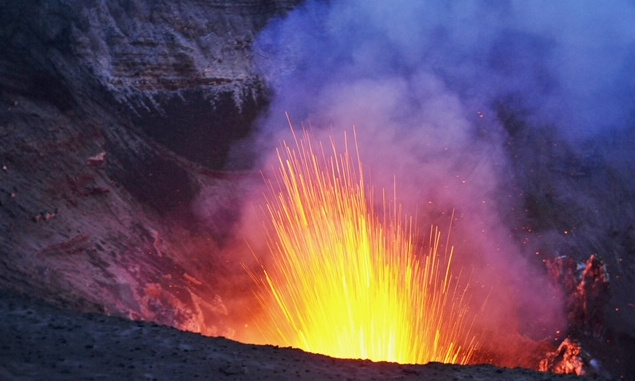
\includegraphics[width=7truecm]{slike/11_photo_vulkan.jpg}\hfill
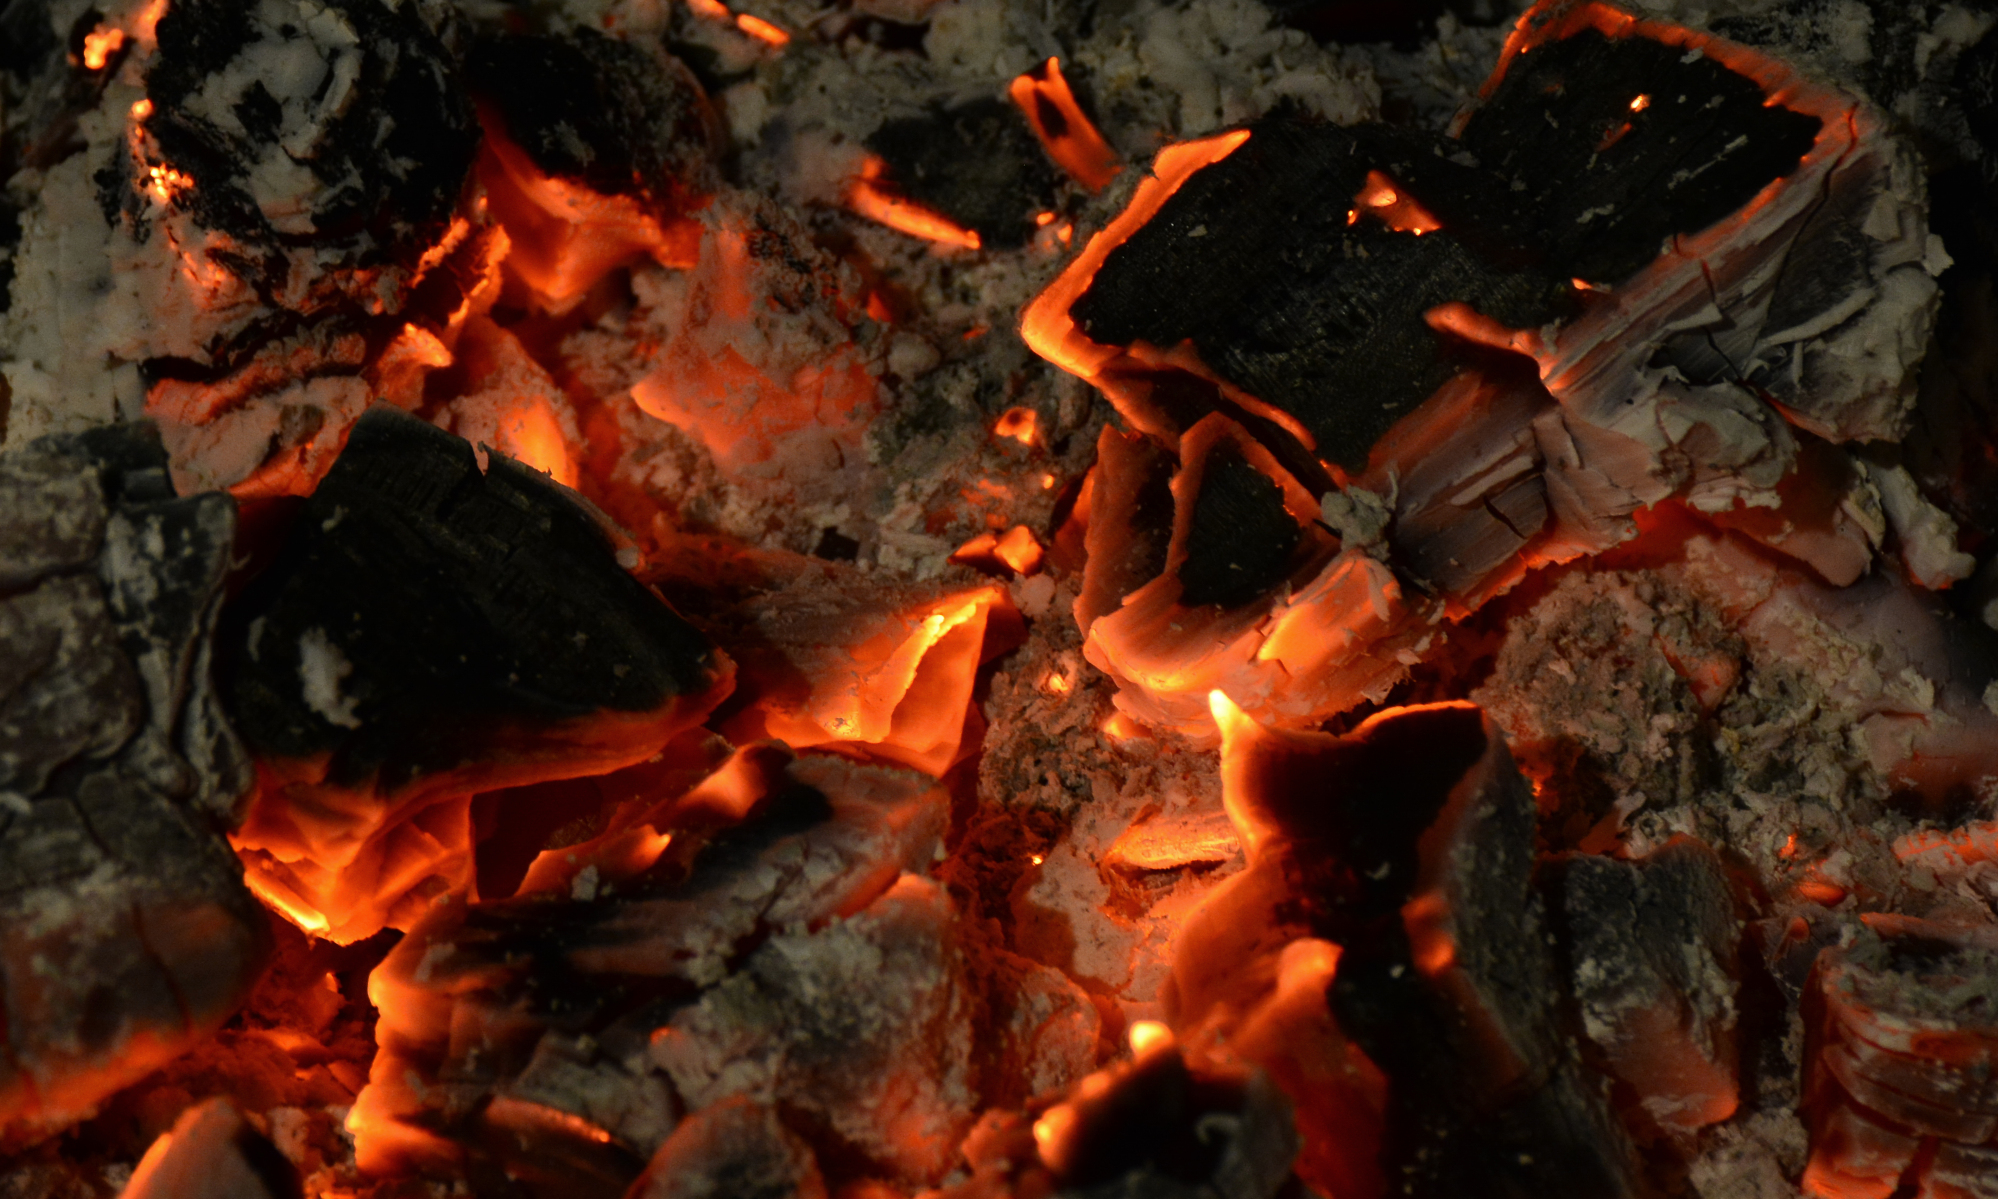
\includegraphics[width=7truecm]{slike/11_photo_zerjavica.jpg} \\ 
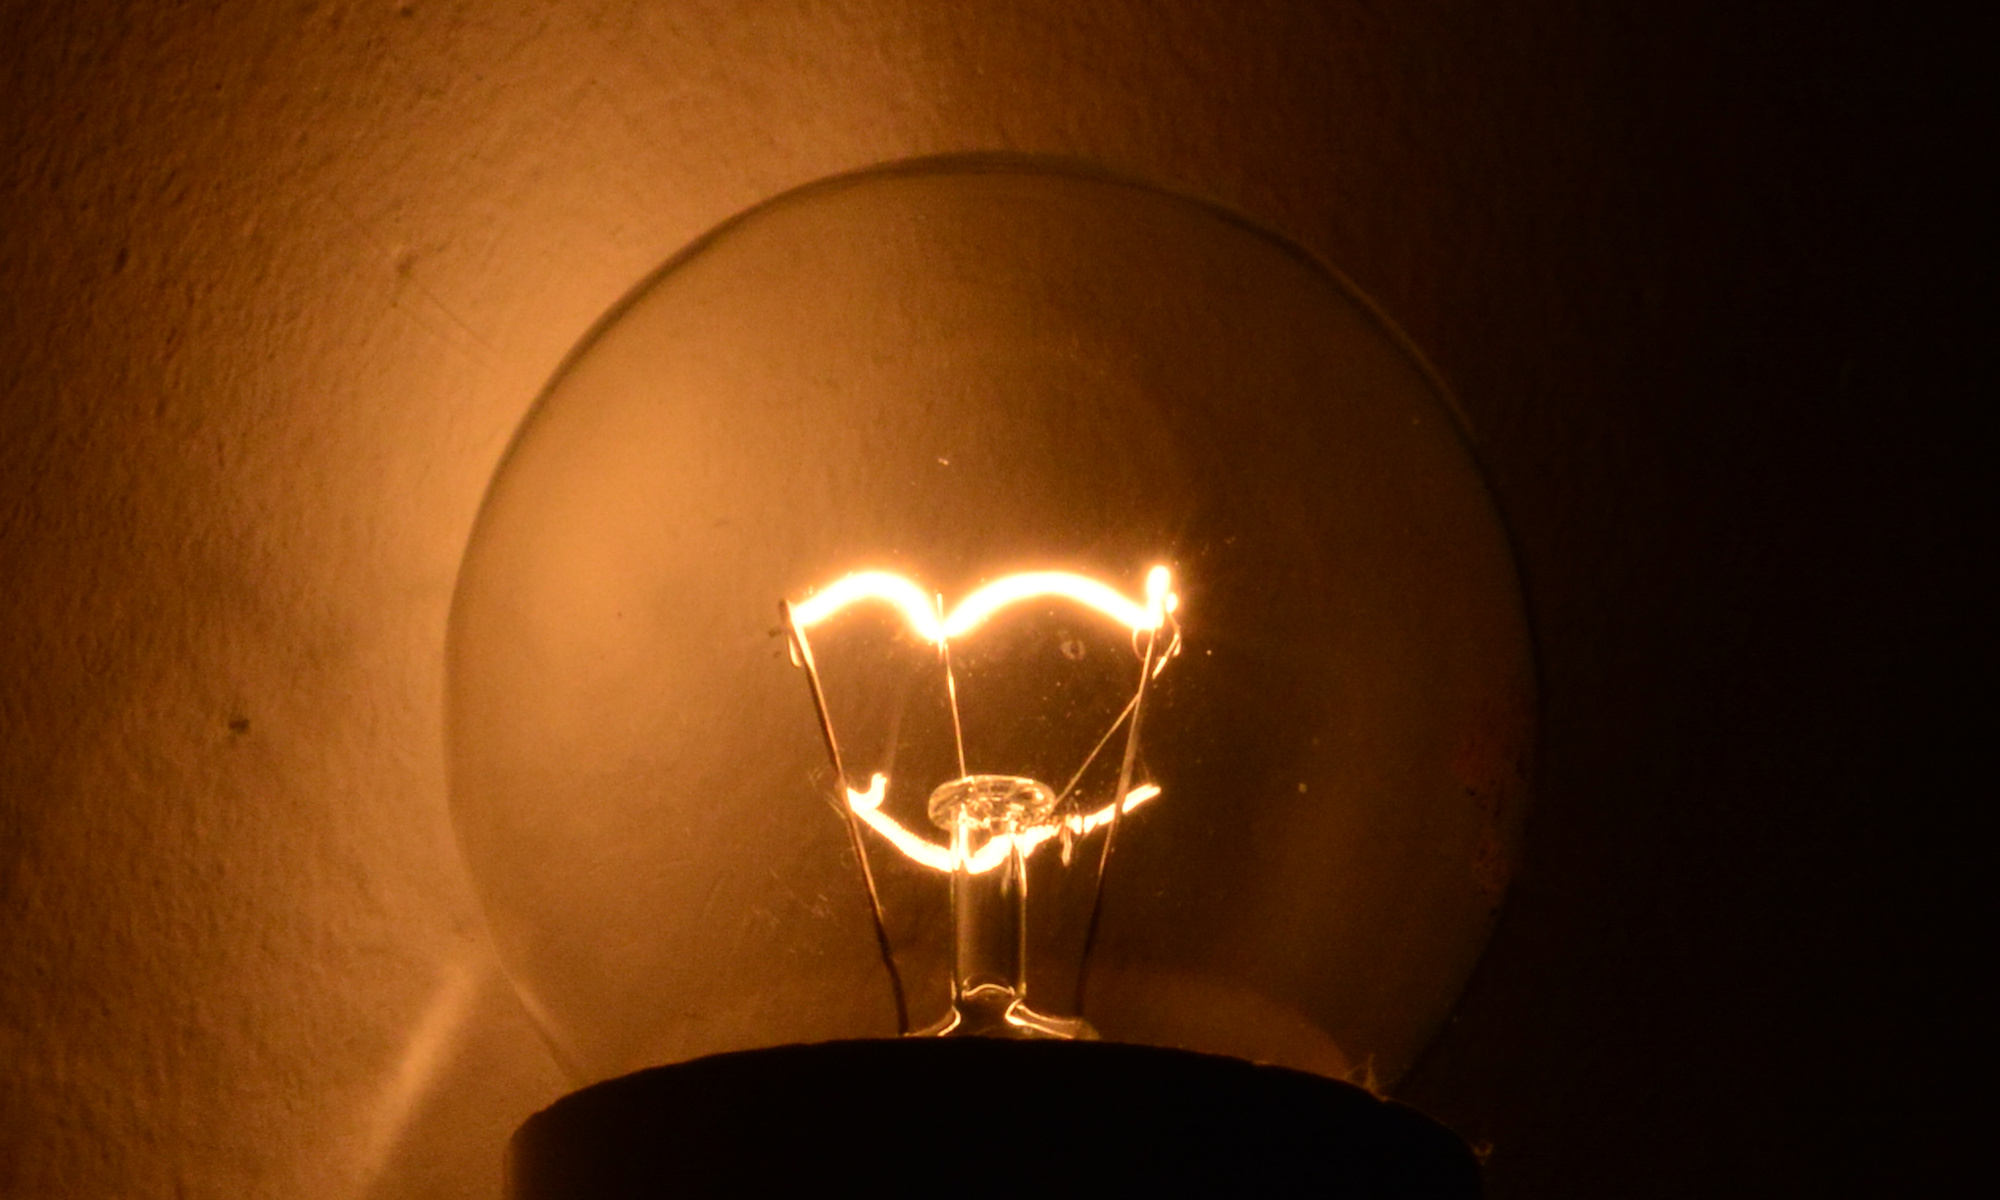
\includegraphics[width=7truecm]{slike/11_photo_zarnica.jpg}\hfill
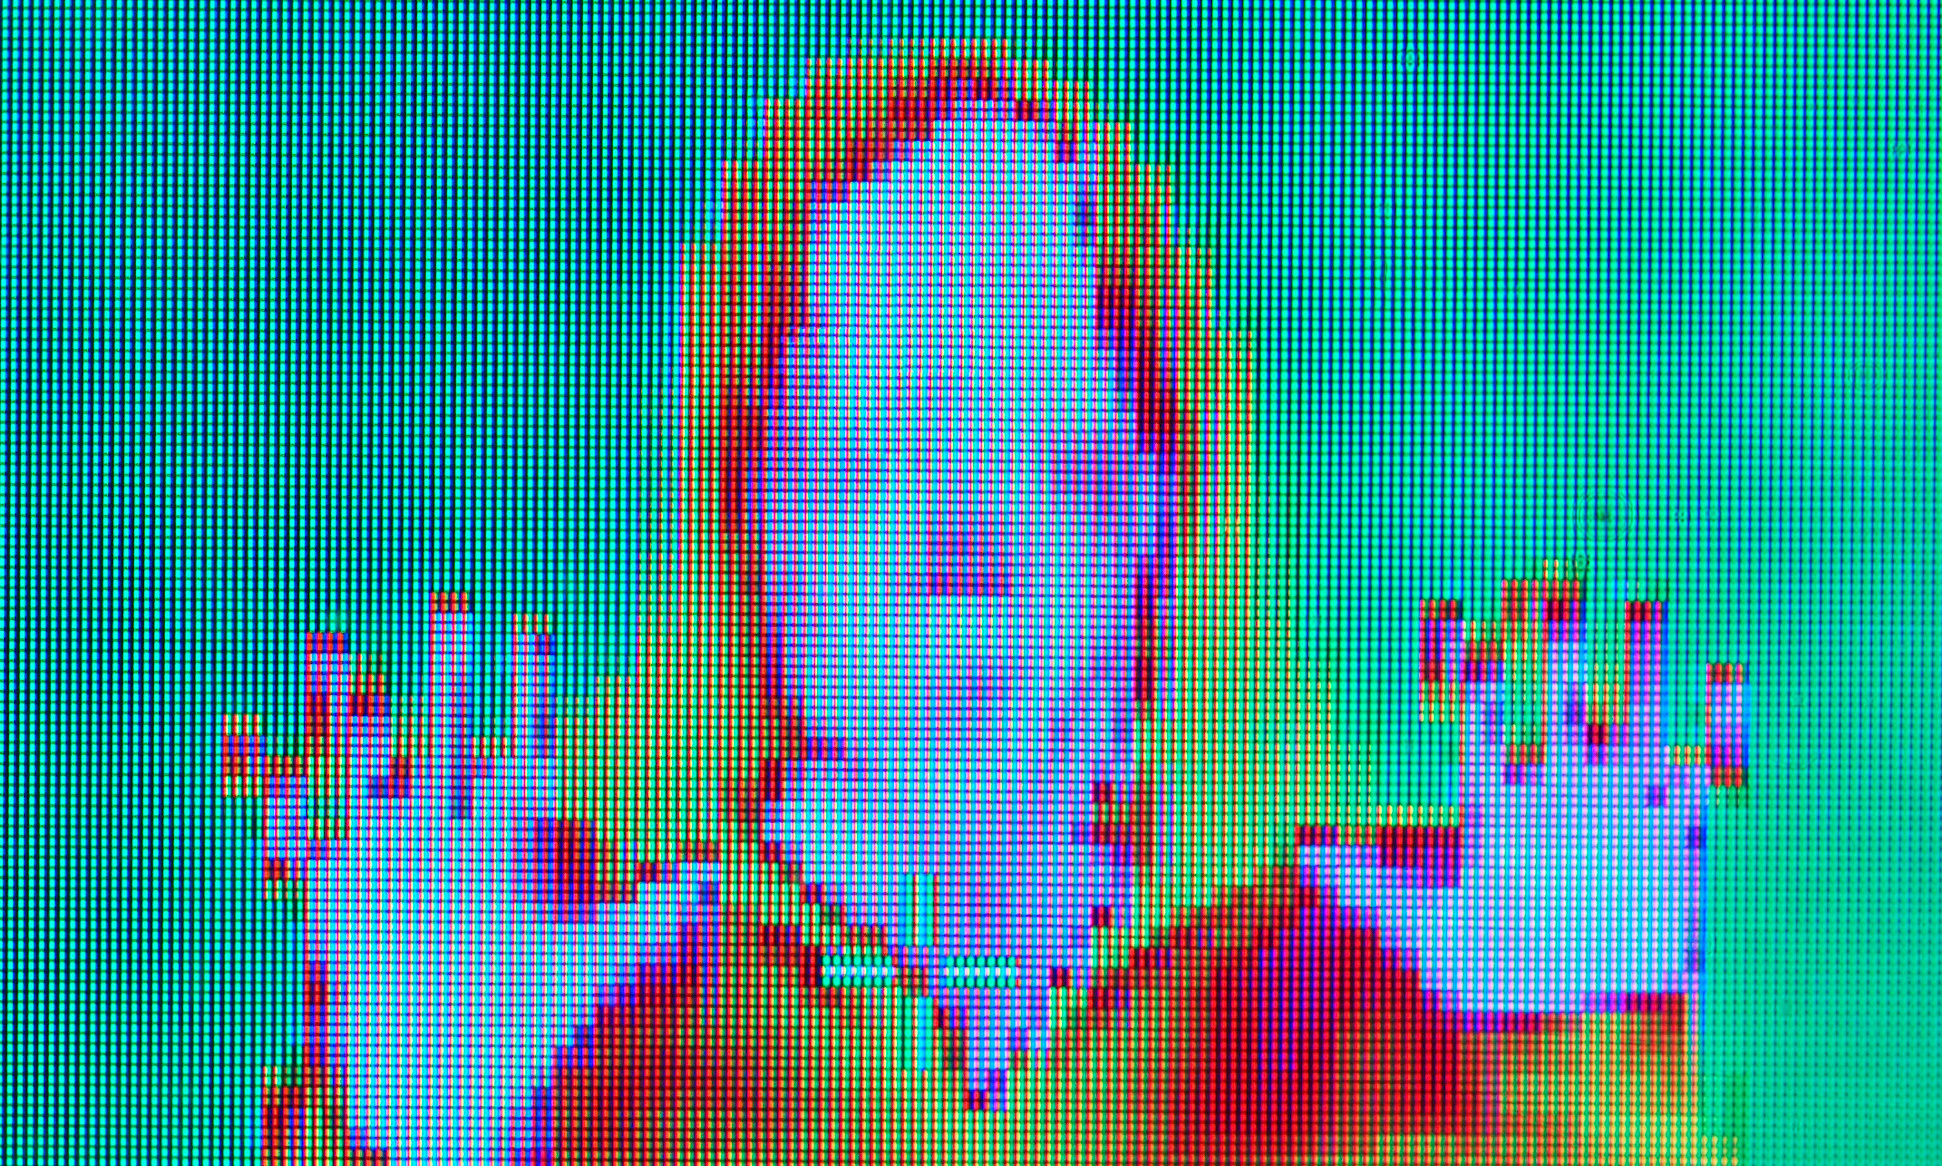
\includegraphics[width=7truecm]{slike/11_photo_IR.jpg} 
\caption{Razgrete snovi sevajo tudi v 
vidnem delu spektra, na primer lava (a), žerjavica (b) ali 
žarilna nitka v žarnici (c). Telesa z nižjo temperaturo sevajo 
predvsem v infrardečem delu spektra~(d), česar z očesom ne zaznamo, z infrardečimi
kamerami pa.}
\label{fig:11_photoPlanck}
\end{figure}

\section{Kvantni opis interakcije svetlobe s snovjo}
Nadaljujmo z obravnavo votline, v kateri so atomi 
in elektromagnetno valovanje v termičnem ravnovesju. 
Zaradi enostavnosti privzamemo, da imajo atomi samo dva 
energijska nivoja, spodnjega (nižjega) pri energiji
$E_1$ in zgornjega (višjega) pri energiji $E_2$. 
Razlika med energijskima nivojema atomov naj ustreza
frekvenci $\omega_{21}$, tako da velja:
\begin{equation}
E_2 -E_1 = \hslash \omega_{21}.
\label{eq:11_07}
\end{equation}
Interakcijo med atomi in elektromagnetnim valovanjem na splošno
opišemo s tremi različnimi procesi: absorpcijo, spontanim
sevanjem in stimuliranim sevanjem (slika~\ref{fig:11_procesi}). 
Oglejmo si te pojave podrobneje.
\vglue3truemm
\begin{figure}[ht!]
\centering
\def\svgwidth{145truemm} 
\input{slike/11_procesi.pdf_tex}
\caption{Trije osnovni procesi interakcije svetlobe s snovjo. Pri absorpciji~(a) 
se foton, označen z rdečim valom, absorbira, atom, označen kot moder krožec, pa 
preide iz nižjega nivoja v višje. Pri spontani emisiji~(b) atom spontano preide 
iz višjega v nižji nivo in pri tem izseva foton. Stimulirana emisija~(c) pa je pojav,
pri katerem vpadni foton sproži prehod atoma iz višjega v nižji nivo, 
izsevani foton pa je identično enak vpadnemu.
}
\label{fig:11_procesi}
\end{figure}

\subsection*{Absorpcija}\index{Absorpcija fotona}
Absorpcija je proces, pri katerem atom absorbira vpadni foton in pri tem 
preide iz nižjega v višje energijsko stanje (slika~\ref{fig:11_procesi}\,a). 
Verjetnost za absorpcijo je močno odvisna od energije vpadnega fotona. Na grobo 
rečemo, da se foton lahko absorbira, če je njegova energija $\hslash \omega$ 
enaka razliki energij med nivojema atoma $E_2-E_1$. Pomemben parameter pri izračunu 
verjetnosti za absorpcijo je tako spektralna gostota energije 
pri frekvenci prehoda med nivojema $u(\omega_{21})$. 
Število atomskih prehodov na časovno enoto je sorazmerno tudi zasedenosti
nižjega nivoja, tako da ga na splošno zapišemo kot:
\begin{equation}
\frac{dN_\mathrm{abs}}{dt} = B_{12}u(\omega_{21}) N_1,
\label{eq:11_08}
\end{equation}
pri čemer sorazmernostno konstanto označimo z $B_{12}$. 

\subsection*{Spontano sevanje}\index{Spontano sevanje}
Spontano sevanje je proces, pri katerem atom, 
ki se nahaja v višjem energijskem nivoju, spontano preide v nižjega
in ob tem izseva foton (slika~\ref{fig:11_procesi}\,b). Energija
izsevanega fotona je enaka razliki energij med atomskima nivojema $E_2-E_1$.

Število spontanih prehodov na časovno enoto je sorazmerno številu
atomov v višjem nivoju in ga zapišemo kot:
\begin{equation}
\frac{dN_\mathrm{sp}}{dt} = A_{21}N_2,
\label{eq:11_09}
\end{equation}
pri čemer smo vpeljali sorazmernostno konstanto $A_{21}$. Tipična vrednost 
za dovoljene prehode je $A_{21}\sim 10^{6}$--$10^8~\si{s^{-1}}$, za prepovedane pa okoli 
štiri velikostne rede manj. 

Inverzna vrednost konstante $A_{21}$\index{Naravni razpadni čas}
ustreza življenjskemu času oziroma naravnemu razpadnemu času višjega
stanja:
\begin{equation}
\tau = \frac{1}{A_{21}}.
\label{eq:11_10}
\end{equation}
Izkazalo se bo, da je v primerjavi s stimuliranim sevanjem spontano sevanje v 
delujočem laserju zanemarljivo, zato ga bomo v računih pogosto zanemarili. 

\begin{remark}
Sorazmernostna konstanta $A_{21}$ opisuje verjetnost za prehod atoma 
iz višjega v nižji energijski nivo s spontanim sevanjem. Podali smo njene približne
numerične vrednosti, uporaba kvantne mehanike pa omogoča tudi njen natančnejši 
izračun. Izračunamo jo lahko z
uporabo Fermijevega zlatega pravila, ki pove verjetnost za prehod 
iz stanja $|2\rangle$ v stanje $|1\rangle$ z dipolnim sevanjem na časovno enoto: 
\begin{equation}
A_{21} = \frac{\omega_{21}^3 \langle 2|e_0\mathbf{r}|1\rangle^2}
{3h \varepsilon_0 c^3}.
\label{eq:11_11}
\end{equation} 
Pri tem so $\omega_{21}$ frekvenca, ki ustreza prehodu med nivojema, $h$ Planckova
konstanta, $\varepsilon_0$ dielektrična konstanta, $c$ svetlobna hitrost in 
$\langle 2|e_0\mathbf{r}|1\rangle$ matrični element za dipolni prehod med stanjema 
$|2\rangle$ in $|1\rangle$.
\end{remark}

\subsection*{Stimulirano sevanje}\index{Stimulirano sevanje}
Tretji način interakcije svetlobe s snovjo je za delovanje laserja
najpomembnejši. Stimulirano sevanje je namreč proces, pri katerem 
vpadni foton sproži prehod atoma iz višjega v nižji energijski nivo, 
ob tem pa nastane foton, ki je povsem enak vpadnemu.
Tako iz enega vpadnega fotona nastaneta dva izhodna fotona, ki potujeta
v isti smeri, imata enako frekvenco, fazo in polarizacijo. Podobno kot absorpcija
lahko tudi ta proces poteče le v primeru, da je energija vpadnega 
fotona enaka razliki energij med atomskima nivojema.

Število prehodov na časovno enoto za stimulirano emisijo zapišemo podobno, 
kot smo zapisali število prehodov na časovno enoto za absorpcijo 
(enačba~\ref{eq:11_08}): 
\begin{equation}
\frac{dN_\mathrm{st}}{dt} = B_{21}u(\omega_{21}) N_2.
\label{eq:11_12}
\end{equation}
Ker mora biti za stimulirano emisijo na začetku atom v višjem stanju, 
je število prehodov sorazmerno $N_2$, sorazmernostni koeficient pa 
označimo z $B_{21}$. Tipične vrednosti
koeficientov so $B_{21}\sim 10^{16}$--$10^{20}~\si{m^3/Js^2}$.

\subsection*{Einsteinovi koeficienti}\index{Einsteinovi koeficienti}
Koeficiente $A$, $B_{12}$ in $B_{21}$, ki smo jih vpeljali kot sorazmernostne
koeficiente pri opisu interakcije svetlobe s snovjo, imenujemo Einsteinovi 
koeficienti. Na preprostem primeru (glej primer~\ref{11_ex_Ei}) bomo pokazali, 
da njihove vrednosti niso neodvisne. Verjetnost za absorpcijo 
je namreč enaka verjetnosti za stimulirano emisijo in velja enakost:
\begin{equation}
B_{12}=B_{21}.
\label{eq:11_13}
\end{equation}
Koeficient bomo zato v nadaljevanju označevali brez indeksov. Poleg tega velja še zveza:
\begin{equation}
\frac{A}{B} = \frac{\hslash \omega_{21}^3}{\pi^2c^3}.
\label{eq:11_14}
\end{equation}
\begin{example}{\bf Zveza med Einsteinovimi koeficienti.}
\label{11_ex_Ei}
Na preprostem primeru bomo pokazali zvezo med Einsteinovimi koeficienti 
(enačbi~\ref{eq:11_13} in \ref{eq:11_14}). Tudi tokrat naj imajo atomi samo 
dva energijska nivoja, nižjega in 
višjega, energija vpadnih fotonov pa naj bo enaka razliki energij med nivojema
$\hslash \omega  = E_2 - E_1= \hslash \omega_{21}$. 
Celotno število atomov je konstantno
in velja $N_1 + N_2 = N$. 

Spreminjanje zasedenosti nižjega nivoja zapišemo kot vsoto treh prispevkov:
\begin{equation}
\frac{dN_1}{dt} = A_{21}N_2 + B_{21}u(\omega_{21})N_2 - B_{12}u(\omega_{21})N_1.
\label{eq:11_15}
\end{equation}
Prvi člen opisuje povečanje zasedenosti nižjega nivoja zaradi 
spontanega sevanja (enačba~\ref{eq:11_09}), drugi člen povečanje 
zaradi stimuliranega sevanja (enačba~\ref{eq:11_12}) in tretji člen
zmanjšanje zasedenosti zaradi absorpcije (enačba~\ref{eq:11_08}).
Za spreminjanje zasedenosti višjega nivoja je izraz zelo podoben, razlikuje
se le v predznaku, saj se vsota zasedenosti obeh nivojev ohranja.

V stacionarnem stanju v termičnem ravnovesju se zasedenosti nivojev 
ne spreminjata in velja:
\begin{equation}
A_{21}N_2 + B_{21}u(\omega_{21})N_2 - B_{12}u(\omega_{21})N_1 = 0.
\label{eq:11_16}
\end{equation}
Od tod izrazimo spektralno gostoto energije:
\begin{equation}
u(\omega_{21}) = \frac{A_{21}N_2}{B_{12}N_1-B_{21}N_2} = 
\frac{A_{21}}{B_{12}N_1/N_2 - B_{21}}.
\label{eq:11_17}
\end{equation}
Upoštevamo Boltzmannovo porazdelitev za zasedenost nivojev 
(enačba~\ref{eq:11_01}) in dobimo:
\begin{equation}
u(\omega_{21}) = \frac{A_{21}}{B_{12}e^{\hslash \omega_{21}/k_B T} - B_{21}}.
\label{eq:11_18}
\end{equation}
Ker je v termičnem ravnovesju tudi elektromagnetno valovanje, ga 
lahko opišemo s Planckovim zakonom. Enačbo~(\ref{eq:11_18}) 
izenačimo z enačbo~(\ref{eq:Planck}):
\begin{equation}
u(\omega_{21}) = \frac{A_{21}/B_{21}}{e^{\hslash \omega_{21}/k_B T}B_{12}/B_{21} - 1} = 
\frac{\hslash \omega^3}{\pi^2c^3}\frac{1}{e^{\hslash \omega/k_bT}-1}
\end{equation}
in primerjamo koeficiente. Da se ujema funkcijska odvisnost v 
imenovalcu, mora veljati:
\begin{equation}
B_{12} = B_{21}.
\label{eq:11_19}
\end{equation}
Preostali faktorji se združijo v obliko:
\begin{equation}
\frac{A_{21}}{B_{21}} = \frac{\hslash \omega_{21}^3}{\pi^2c^3},
\label{eq:11_20}
\end{equation}
s čimer smo pokazali še veljavnost enačbe~(\ref{eq:11_14}).

Parametre $A$ in $B$ imenujemo po Albertu Einsteinu, ki je že leta\index{Einstein, Albert} 
1916 proučeval interakcije svetlobe s snovjo in predlagal opisani model s tremi osnovnimi procesi. 
Na podlagi modela je napovedal možnost ojačenja svetlobe s stimulirano 
emisijo in tako postavil teoretično utemeljitev delovanja laserjev.
Do prvega delujočega laserja je potem minilo še  več kot 40 let. 

\end{example}

\section{Interakcija svetlobe s snovjo v optičnem resonatorju}
Optični resonatorji so naprave, znotraj katerih lahko vzbudimo\index{Optični resonator}
stoječe elektromagnetno valovanje. Resonatorje navadno poznamo iz glasbe,
za svetlobo pa si lahko resonatorje mislimo kot zaprto škatlo
z zrcali na notranjih straneh, od katerih se svetloba 
odbija (slika~\ref{fig:11_resonator}\,a).
Frekvence vzbujenih stoječih valovanj (lastnih nihanj) so točno 
določene z geometrijo resonatorja in robnimi pogoji na njegovih 
stenah (slika~\ref{fig:11_resonator}\,b).
Frekvence lastnih nihanj imenujemo tudi resonančne frekvence. 
Zaradi izgub v resonatorju črte v resonančnem spektru niso 
neskončno ozke, temveč imajo neko končno širino
(slika~\ref{fig:11_resonator}\,c).
\vglue2truemm
\begin{figure}[ht!]
\centering
\def\svgwidth{140truemm} 
\input{slike/11_resonator.pdf_tex}
\caption{Najpreprostejši primer optičnega resonatorja sta 
dve vzporedni zrcali, med katerima se svetloba odbija~(a). Stoječa
valovanja, ki jih vzbudimo v resonatorju, so njegova lastna nihanja~(b). 
Spekter svetlobe v resonatorju je diskreten, vendar so posamezne 
črte zaradi izgub razširjene (c).
}
\label{fig:11_resonator}
\end{figure}

Po drugi strani tudi energijska razlika med posameznima atomskima nivojema 
ni povsem točno določena. Zaradi končnega razpadnega časa 
(enačba~\ref{eq:11_10}) ima spekter prehoda neko končno širino. Tako imenovano
atomsko spektralno črto opišemo s funkcijo $g(\omega)$,\index{Atomska spektralna črta}
ki je Lorentzeve ali Gaussove oblike okoli osrednje
frekvence prehoda $\omega_{21}$. Zanjo velja:
\begin{equation}
\int_{-\infty}^\infty g(\omega) d\omega = 1.
\label{eq:11_21}
\end{equation}
Spekter sevanja črnega telesa, ki smo ga spoznali v prejšnjem razdelku 
(enačba~\ref{eq:Planck}), je širok. Zato lahko privzamemo, da je\index{Spekter!{Planckov}}
znotraj atomske spektralne širine približno konstanten 
in enak $u(\omega_{21})$ (glej sliko~\ref{fig:11_g}\,a).
To smo tudi upoštevali v zapisu enačb za absorpcijo (enačba~\ref{eq:11_08})
in stimulirano sevanje (enačba~\ref{eq:11_12}). 

Kadar obravnavamo svetlobo v resonatorju, je njen spekter zelo drugačen 
od spektra črnega telesa, saj je sestavljen iz ozkih diskretnih črt.
Pri opisu interakcije svetlobe s snovjo v resonatorju je zato treba 
upoštevati prekrivanje resonatorskega spektra in 
spektra atomskega sistema. Oba sta ozka z neko končno širino, vendar 
je širina resonanc v resonatorju navadno dosti ožja od naravne širine 
emisijske oziroma absorpcijske črte (slika~\ref{fig:11_g}\,b).
\vglue2truemm
\begin{figure}[ht!]
\centering
\def\svgwidth{130truemm} 
\input{slike/11_g.pdf_tex}
\caption{Primerjava atomske spektralne črte (modra) in svetlobnega spektra (rdeča): (a)
spekter sevanja črnega telesa $u(\omega)$ je bistveno širši 
od atomske spektralne črte $g(\omega)$; (b) spekter svetlobe iz 
resonatorja $u(\omega)$ je navadno bistveno ožji od atomske 
spektralne črte $g(\omega)$. V laserjih velja drugi primer.
}
\label{fig:11_g}
\end{figure}

Na splošno moramo pri zapisu izrazov za absorpcijo in stimulirano emisijo 
upoštevamo širini obeh črt. Število prehodov za absorpcijo je tako:
\begin{equation}
\frac{dN_\mathrm{abs}}{dt} = BN_1 \int_{-\infty}^{\infty} g(\omega) u(\omega) d\omega
\label{eq:11_22}
\end{equation}
in za stimulirano emisijo:
\begin{equation}
\frac{dN_\mathrm{st}}{dt} = BN_2 \int_{-\infty}^{\infty} g(\omega) u(\omega) d\omega.
\label{eq:11_23}
\end{equation}
Prvi skrajni primer, ko je bila širina spektra črnega telesa bistveno širša
od atomske spektralne črte, smo že opisali (enačbi~\ref{eq:11_08} in \ref{eq:11_12}). 
Poglejmo zdaj še drugo skrajnost, 
ko je spektralna širina resonančnih črt, podana s funkcijo $u(\omega)$, bistveno 
ožja od atomske spektralne črte, podane z $g(\omega)$. V tem primeru 
lahko privzamemo, da je vrednost $g(\omega)$ znotraj integrala konstantna in 
upoštevamo le njeno vrednost pri izbrani resonančni frekvenci $\omega_R$.
Integral tudi v tem primeru preprosto izračunamo:
\begin{equation}
\int_{-\infty}^{\infty} g(\omega) u(\omega) d\omega = g(\omega_R) \int_{-\infty}^{\infty}
u(\omega) d\omega = g(\omega_R) w,
\label{eq:11_24}
\end{equation}
pri čemer je $w$ gostota energije elektromagnetnega valovanja. 
Število prehodov za absorpcijo na časovno enoto v tem približku zapišemo kot:
\begin{equation}
\frac{dN_\mathrm{abs}}{dt} = B N_1 g(\omega_R) w
\label{eq:11_25}
\end{equation}
in za stimulirano sevanje kot:
\begin{equation}
\frac{dN_\mathrm{st}}{dt} = B N_2 g(\omega_R) w.
\label{eq:11_26}
\end{equation}
Ponovimo: $g(\omega_R)$ je vrednost atomske spektralne črte $g$ pri 
frekvenci $\omega_R$, ki ustreza monokromatskemu resonančnemu 
elektromagnetnemu valovanju znotraj resonatorja, $w$ pa je gostota
energije valovanja pri resonančni frekvenci $\omega_R$. 
\vglue-2truemm
\begin{remark}
Kljub temu da ima funkcija $g(\omega)$ navadno Lorentzovo ali Gaussovo 
obliko, jo pri računanju zaradi preprostosti velikokrat nadomestimo 
s škatlasto funkcijo. Njena vrednost je izven nekega ustreznega 
intervala $\Delta \omega$ enaka 0, znotraj tega intervala pa ima 
funkcija konstantno vrednost $g = 1/\Delta \omega$. Tipične vrednosti
so $\Delta \omega \sim 10^9$--$10^{12}~\si{Hz}$.
\end{remark}

\section{Ojačevanje svetlobe}\index{Ojačevanje svetlobe}
Fotoni, ki vpadajo na snov, se lahko v njej absorbirajo ali v njej sprožijo
stimulirano emisijo, pri čemer absorpcija fotonov vpadni svetlobni tok 
zmanjšuje, stimulirana emisija pa ga povečuje. Pri pravih pogojih lahko
dosežemo, da je moč izhodne svetlobe večja od moči vpadne svetlobe in tak
sistem imenujemo optični ojačevalnik.

Naj svetloba vpada vzdolž osi $z$ pod pravim kotom na tanko plast snovi. 
Debelina plasti naj bo $dz$, njena prostornina pa $V = S dz$. V plasti naj 
bo $N_1$ atomov v nižjem energijskem stanju in $N_2$ v višjem. 
Moč vpadne svetlobe naj bo $P$ (slika~\ref{fig:11_absorpcija}). Ko 
svetloba prehaja skozi snov, se njena moč zmanjšuje zaradi absorpcije 
in povečuje zaradi stimuliranega sevanja. Spontano sevanje 
zanemarimo, saj je spontano izsevana svetloba enakomerno 
porazdeljena v vseh smereh in le zanemarljivo majhen delež je usmerjen 
vzdolž osi $z$. Obravnavajmo primer, ko je spekter vpadne svetlobe
zelo ozek, na primer iz optičnega resonatorja.
\begin{figure}[ht!]
\centering
\def\svgwidth{70truemm} 
\input{slike/11_absorpcija.pdf_tex}
\caption{Svetlobna moč se zmanjšuje zaradi absorpcije in povečuje
zaradi stimulirane emisije.}
\vglue-4truemm
\label{fig:11_absorpcija}
\end{figure}

Sprememba svetlobne moči ob prehodu skozi plast snovi je:
\begin{equation}
dP = \hslash \omega \left(\frac{dN_\mathrm{st}}{dt}- 
\frac{dN_\mathrm{abs}}{dt}\right)\!\!,
\label{eq:11_27}
\end{equation}
pri čemer smo upoštevali povečanje zaradi stimulirane emisije in zmanjšanje
zaradi absorpcije, prispevek spontanega sevanja pa smo že zanemarili.
Z uporabo enačb~(\ref{eq:11_25} in \ref{eq:11_26}) dobimo:
\begin{equation}
dP = 
\hslash \omega \left(N_2Bg(\omega) w - N_1Bg(\omega)w\right) = 
\hslash \omega\,B g(\omega) w\, (N_2 - N_1).
\label{eq:11_28}
\end{equation}
Upoštevamo zvezo $w = j/c$ (enačba~\ref{eq:j}) in enačbo delimo s $S$:
\begin{equation}
dj = \hslash \omega\,B g(\omega) \frac{j}{c}\frac{(N_2-N_1)}{V}dz.
\label{eq:11_29}
\end{equation}
Zapisano enačbo lahko v poenostavljeni obliki zapišemo kot:
\boxeq{eq:ojacenje}{
dj = \sigma\,\frac{N_2-N_1}{V}jdz = \gamma j dz.
}
Pri tem smo vpeljali presek za absorpcijo in stimulirano 
emisijo:\index{Presek za absorpcijo in stimulirano emisijo}
\begin{equation}
\sigma (\omega)= \frac{\hslash \omega\, Bg(\omega)}{c}.
\label{eq:11_30}
\end{equation}
Presek $\sigma$ je odvisen od snovi in od frekvence vpadnega valovanja. 
Tipične vrednosti so $\sigma \sim 10^{-20}~\si{m^2}$.

Drugi parameter, ki smo ga vpeljali v enačbi~(\ref{eq:ojacenje}), 
je koeficient ojačenja $\gamma$:\index{Koeficient ojačenja}
\begin{equation}
\gamma = \sigma \,\frac{N_2-N_1}{V}.
\label{eq:11_31}
\end{equation}
Ta parameter je odvisen od zasedenosti posameznih  nivojev. 
Kadar je snov v termičnem ravnovesju in velja $N_2 < N_1$, je $\gamma <0$
in svetlobna moč se po prehodu skozi snov zmanjša. 

Da dosežemo
ojačenje svetlobnega toka, mora biti koeficient ojačenja $\gamma >0$. 
Iz enačbe~(\ref{eq:11_31}) sledi, da je ta pogoj izpolnjen, kadar je $N_2>N_1$.
Ojačenje svetlobe v snovi lahko dosežemo le v primeru, ko je zasedenost
višjega nivoja večja od zasedenosti nižjega nivoja. Tako neravnovesno 
stanje imenujemo stanje obrnjene zasedenosti. V termičnem ravnovesju\index{Obrnjena zasedenost}
obrnjene zasedenosti ne moremo doseči, zato moramo za ojačenje svetlobe
sistem atomov vzdrževati v neravnovesnem stanju z dovajanjem energije od zunaj.

\section{Trinivojski sistemi}\index{Trinivojski sistem}
Da lahko v nekem sistemu svetlobo ojačujemo, moramo med 
dvema nivojema doseči obrnjeno zasedenost. Izkaže se, da v dvonivojskem 
sistemu s še tako močnim črpanjem obrnjene zasedenosti ne moremo doseči, 
ampak moramo v interakcijski proces med snovjo in svetlobo vključiti 
vsaj tri atomske nivoje. Takrat govorimo o trinivojskem sistemu 
(slika~\ref{fig:11_3nivojski}).
\begin{figure}[ht!]
\centering
\def\svgwidth{100truemm} 
\input{slike/11_3nivojski.pdf_tex}
\caption{Obrnjeno zasedenost dosežemo v vsaj trinivojskem sistemu (a). Energijske
nivoje označimo z $E_0$, $E_1$ in $E_2$, z istimi indeksi tudi ustrezne 
zasedenosti $N_0$, $N_1$ in $N_2$, 
prehode med nivoji (absorpcijo, spontano in stimulirano emisijo) pa s pripadajočimi
Einsteinovimi koeficienti $A$ in $B$. Parameter $r$ označuje črpanje. Primer
trinivojskega sistema, v katerem je laserski prehod med prvim in drugim vzbujenim
nivojem (b).
}
\vglue-5truemm
\label{fig:11_3nivojski}
\end{figure}

Naj bo celotno število atomov v sistemu $N$, zasedenosti posameznih nivojev pa 
označimo z indeksom nivoja. Potem velja:\index{Zasedenost nivoja}
\begin{equation}
N = N_0 + N_1 + N_2.
\label{eq:11_32}
\end{equation}
Pri obravnavi bomo privzeli, da je zasedenost osnovnega (najnižjega) 
nivoja bistveno večja od zasedenosti drugih dveh nivojev $N_0 \gg N_1, N_2$ 
in zato rekli, da velja $N_0 \approx N$. 

Na sistem trinivojskih atomov naj vpada svetloba s frekvenco:
\begin{equation}
\omega_{21} = \frac{E_2-E_1}{\hslash},
\label{eq:11_33}
\end{equation}
ki ustreza energijski razliki med prvim in drugim vzbujenim stanjem.  Če želimo
vpadno svetlobo ojačevati, moramo doseči obrnjeno zasedenost med nivojema 1 in 2.
To naredimo z zunanjim črpalnim mehanizmom, s katerim vzbujamo atome 
iz osnovnega v drugi vzbujeni nivo.

Črpanje neodvisno od črpalnega mehanizma
opišemo s koeficientom $r$:
\begin{equation}
\frac{dN_2}{dt} = r\, N_0.
\label{eq:11_34}
\end{equation}
Zasedbene enačbe za vse tri nivoje zapišemo z upoštevanjem prehodov med njimi. 
Poglejmo podrobneje spreminjanje zasedenosti drugega vzbujenega nivoja 
(slika~\ref{fig:11_3nivojski}\,a). Zasedenost
se povečuje zaradi črpanja ($r$) in zmanjšuje zaradi spontanih
prehodov v prvo vzbujeno ($A_{21}$) in v osnovno stanje ($A_{20})$. V prisotnosti
svetlobe se zasedenost povečuje še zaradi absorpcije ($B_{12}$) in zmanjšuje
zaradi stimuliranega sevanja ($B_{21}$). Vse prispevke združimo v eno enačbo, 
nato naredimo podoben razmislek še za ostala dva nivoja. Dobimo sistem enačb:
\begin{align}
\frac{dN_2}{dt} &= rN_0 - A_{20}N_2 - A_{21}N_2 + B_{21}w(\omega_{21})g(\omega_{21}) 
(N_1-N_2),\label{eq:11_35}\\
\frac{dN_1}{dt} &= - A_{10}N_1 + A_{21}N_2 - B_{21}w(\omega_{21})g(\omega_{21}) 
(N_1-N_2),\label{eq:11_36}\\
\frac{dN_0}{dt} &= - rN_0 + A_{20}N_2 + A_{10}N_1.\label{eq:11_37}
\end{align}
Vidimo, da vsak prehod v sistemu enačb nastopa dvakrat: enkrat s pozitivnim 
in enkrat z negativnim predznakom. Vsota vseh treh enačb je posledično enaka 
nič, kar se ujema z zahtevo, da je vsota zasedenosti konstantna. Za reševanje
sistema zato zadošča obravnava le dveh enačb. Poleg tega lahko že takoj 
naredimo nekaj poenostavitev. Namesto $N_0$ vstavimo $N$, ki je konstanten, 
in brez škode zanemarimo spontane prehode iz drugega vzbujenega 
nivoja v osnovnega ($A_{20}$). Spontanih prehodov iz prvega v osnovni 
nivo ($A_{10}$) seveda ne smemo zanemariti, saj je to ključni
mehanizem, ki prazni nižji vzbujeni nivo.

Zanima nas stacionarno stanje, ko so časovni odvodi enaki nič. 
Iz enačbe~(\ref{eq:11_37}) dobimo:
\begin{equation}
N_1 \approx \frac{rN}{A_{10}}.
\label{eq:11_38}
\end{equation}
Enačba~(\ref{eq:11_36}) se v stacionarnem stanju prepiše v:
\begin{equation}
\left(A_{21}+ B_{21}w(\omega_{21})g(\omega_{21})\right)N_2 = 
\left(A_{10}+ B_{21}w(\omega_{21})g(\omega_{21})\right)N_1.
\label{eq:11_39}
\end{equation}
Iz enačb~(\ref{eq:11_38} in \ref{eq:11_39}) izrazimo razliko 
zasedenosti vzbujenih nivojev in dobimo:
\begin{equation}
N_2-N_1 = \frac{A_{10}-A_{21}}{A_{21} + B_{21}w(\omega_{21})g(\omega_{21})}
\cdot \frac{rN}{A_{10}}.
\label{eq:11_40}
\end{equation}
Za dosego obrnjene zasedenosti v trinivojskem sistemu mora torej 
veljati $A_{10}>A_{21}$: verjetnost za prehod iz prvega vzbujenega nivoja v 
osnovni nivo mora biti večja od verjetnosti za prehod iz 
drugega vzbujenega v prvi vzbujeni nivo. Povedano drugače: 
za dosego obrnjene zasedenosti se mora srednji nivo 
prazniti hitreje od najvišjega nivoja. 

V praksi navadno uporabljamo sisteme, v katerih je $A_{10}\gg A_{21}$.
V tem primeru lahko izraz za obrnjeno zasedenost (enačba~\ref{eq:11_40}) 
še dodatno poenostavimo in dobimo:
\begin{equation}
N_2-N_1 = \frac{rN}{A_{21}}\cdot\frac{1}{1+B_{21}w(\omega_{21})g(\omega_{21})/A_{21}}.
\label{eq:11_41}
\end{equation}
Upoštevamo zvezo $w = j/c$ in zapišemo:
\begin{equation}
N_2-N_1 = \frac{rN}{A_{21}}\cdot\frac{1}{1+\frac{B_{21}g(\omega_{21})}{A_{21}c}j} = 
\frac{rN}{A_{21}}\cdot \frac{1}{1+j/j_s}.
\label{eq:11_42}
\end{equation}
Vpeljali smo saturacijsko gostoto toka:\index{Saturacijska gostota toka}
\begin{equation}
j_s = \frac{A_{21}c}{B_{21}g(\omega_{21})},
\label{eq:11_42a}
\end{equation}
ki je odvisna od snovi in od frekvence vpadne svetlobe. Iz enačbe~(\ref{eq:11_42}) razberemo, 
da dosežemo pri  dani saturacijski gostoti toka $j_s$ večjo obrnjeno zasedenost
pri močnejšem črpanju~$r$.

Z upoštevanjem izraza za presek za absorpcijo in stimulirano emisijo 
(enačba~\ref{eq:11_30}) lahko saturacijsko gostoto toka zapišemo kot:
\begin{equation}
j_s = \hslash \omega \frac{A_{21}}{\sigma}
\label{eq:11_42b}
\end{equation}
in na grobo ocenimo velikostni red $j_s \sim 10^7~\si{W/m^2}$. 

Vstavimo zdaj izračunano obrnjeno zasedenost (enačba~\ref{eq:11_42}) v enačbo za 
optično ojačevanje (enačba~\ref{eq:ojacenje}):
\begin{equation}
dj = \sigma (\omega_{21})\frac{rN}{VA_{21}}\cdot \frac{1}{1 + j/j_s}j\,dz.
\label{eq:11_43}
\end{equation}
Vpeljemo koeficient ojačenja pri majhnih gostotah vpadnega\index{Koeficient ojačenja!{pri majhnih $j$}}
energijskega toka:
\begin{equation}
G = \sigma(\omega_{21})\frac{rN}{VA_{21}}
\label{eq:11_44}
\end{equation}
in optično ojačevanje strnjeno zapišemo v obliki:
\boxeq{eq:3ojacevanje}{
dj = \frac{G j\,dz}{1+j/j_s}.
}
Enačbo~(\ref{eq:3ojacevanje}) integriramo:
\begin{equation}
\int_{j_0}^j \frac{dj}{j}\left(1 + j/j_s\right) = \int_0^z G\, dz,
\label{eq:11_45}
\end{equation}
pri čemer $j_0$ označuje vpadno gostoto svetlobnega toka, $j$ pa po 
prepotovani razdalji $z$. Dobimo:
\begin{equation}
\ln\frac{j}{j_0} + \frac{j-j_0}{j_s} = Gz.
\label{eq:11_46}
\end{equation}
Zapisana enačba podaja spreminjanje gostote
energijskega toka v odvisnosti od prepotovane razdalje v snovi. Odvisnosti
$j(z)$ ne moremo enostavno zapisati, lahko pa jo narišemo.
Na sliki~\ref{fig:11_ojacenje} je prikazano naraščanje
relativne gostote svetlobnega toka $j(z)/j_0$ v odvisnosti od $z$ pri 
izbrani vrednosti saturacijskega toka $j_s/j_0 = 20$.
\begin{figure}[ht!]
\centering
\def\svgwidth{65truemm} 
\input{slike/11_ojacenje.pdf_tex}
\caption{Ojačenje svetlobe v trinivojskem sistemu z obrnjeno zasedenostjo.
Pri majhnih vpadnih močeh je naraščanje eksponentno, pri velikih močeh 
pa linearno, saj se ojačenje nasiti.
}
\label{fig:11_ojacenje}
\vglue-3truemm
\end{figure}

Naraščanje gostote svetlobnega toka (enačba~\ref{eq:11_46}) 
lahko preprosto zapišemo v limitnih primerih zelo majhnih ali 
zelo velikih vrednosti $j_0$. 
Kadar so vpadne moči majhne in je $j \ll j_s$, drugi člen
na levi strani enačbe~(\ref{eq:11_46}) zanemarimo in ostane eksponentno 
naraščajoča odvisnost od dolžine prepotovane poti po snovi:
\begin{equation}
j = j_0e^{Gz}.
\label{eq:11_47}
\end{equation}
Eksponentno naraščanje vidimo na sliki~\ref{fig:11_ojacenje}
pri majhnih vrednostih $j$. 

Pri velikih močeh vpadne svetlobe, za katere velja $j \gg j_s$, 
zanemarimo prvi člen na levi strani enačbe~(\ref{eq:11_46}) in dobimo:
\begin{equation}
j = j_0 + Gj_s\, z.
\label{eq:11_48}
\end{equation}
Naraščanje svetlobne moči pri velikih vrednostih torej preide iz 
eksponentnega v linearno obnašanje. Opisani pojav imenujemo 
nasičenje ojačenja.\index{Nasičenje ojačenja}

Svetloba se v snovi, v kateri je vzpostavljena
obrnjena zasedenost, ojačuje, saj je stimulirane emisije več
kot absorpcije. Izsevani fotoni sprožijo nadaljnje prehode
in pri majhnih vrednostih gostote svetlobnega toka je  
naraščanje eksponentno. Pri velikih svetlobnih močeh začne
vzbujenih atomov, ki bi lahko izsevali svetlobo, primanjkovati.
V skrajnem primeru stimulirano sevajo prav vsi vzbujeni atomi in 
svetlobna moč narašča le še linearno s prepotovano razdaljo. 
Parameter, ki pove, 
ali se svetloba eksponentno ojačuje ali njena
intenziteta narašča linearno, je ravno saturacijska
gostota svetlobnega toka $j_s$ (enačba~\ref{eq:11_42a}). 

Vrnimo se k enačbi~(\ref{eq:11_48}) in produktu $Gj_s$. Vstavimo enačbi
za koeficient ojačenja pri nizkih močeh (enačba~\ref{eq:11_44}) 
in saturacijsko gostoto (enačba~\ref{eq:11_42b}). Dobimo:
\begin{equation}
Gj_s = \sigma \frac{r N}{V A_{21}} 
\cdot \frac{\hslash \omega_{21} A_{21}}{\sigma}=
\hslash \omega_{21}\frac{rN}{V}.
\label{eq:11_49}
\end{equation}
Povečanje gostote svetlobnega toka v plasti debeline $dz$ potem zapišemo kot:
\begin{equation}
dj = \hslash \omega_{21}\frac{rN}{V}dz,
\label{eq:11_50}
\end{equation}
kar pomeni, da v izbrani plasti snovi vsi atomi, 
ki jih s črpalnim mehanizmom vzbudimo v drugi vzbujeni
nivo, na osnovi stimulirane emisije prispevajo dodatni 
svetlobni tok k vpadnemu elektromagnetnemu valovanju.
Takrat torej vso razpoložljivo energijo sistema počrpamo 
in ojačenje se nasiti. 

\section{Laser}\index{Laser}
Laser je naprava, v kateri izkoristimo stimulirano sevanje\index{Simulirano sevanje} 
za nastanek močne koherentne in monokromatske izhodne svetlobe. Dodatna odlika
laserske svetlobe je njena ozka usmerjenost (majhna divergenca svetlobnega snopa)
in zelo velika gostota svetlobnega toka v snopu.

Laser\footnote{Laser je kratica za {\it Light Amplification by Stimulated
Emission of Radiation}, to je ojačevanje svetlobe s stimuliranim sevanjem.} 
v grobem sestavljajo trije osnovni sestavni deli: ojačevalno sredstvo,
v katerem se svetloba ojačuje, črpalni sistem, ki vzdržuje obrnjeno zasedenost
v ojačevalnem sredstvu, in resonator, ki zagotavlja prevlado stimuliranega sevanja
(slika~\ref{fig:11_laser}).

\begin{figure}[ht!]
\centering
\def\svgwidth{100truemm} 
\input{slike/11_laser.pdf_tex}
\caption{Shema laserja s tremi poglavitnimi sestavnimi deli (zgoraj): 
ojačevalnim sredstvom, črpalnim mehanizmom in resonatorjem. Odbojnost 
izhodnega zrcala $\mathcal{R}_2$ je manjša od $100\%$, da lahko svetloba 
izhaja iz resonatorja. Spodaj: fotografija starejšega helij-neonskega laserja,\index{Laser!{He-Ne}}
narejenega v Sloveniji. Ohišje laserja je odprto, da se vidi notranje elemente.
}
\label{fig:11_laser}
\end{figure}

Ojačevalno sredstvo je najznačilnejši del laserja, saj je od njega odvisna 
valovna dolžina izhodne svetlobe. Laserje zato tudi navadno poimenujemo
po snovi, iz katere je ojačevalno sredstvo.
Ojačevalno sredstvo je lahko plin, trdna snov ali tekočina.  
Šolski laserji so plinski helij-neonski (He-Ne) laserji, ki oddajajo\index{Laser!{He-Ne}} 
rdečo svetlobo pri $632,8~\si{nm}$. V njih je ojačevalno sredstvo
mešanica plinov helija in neona. Danes najbolj razširjenji laserji so\index{Laser!{diodni}}
diodni laserji, v katerih se svetloba ojačuje na p-n spoju polprevodnika. 
Valovne dolžine diodnih laserjev sežejo od $\sim 375~\si{nm}$ do več 
$\si{\micro\meter}$, odvisno od polprevodnika in njegovih primesi.

Črpalni mehanizem je odvisen od izbire ojačevalnega sredstva. Črpamo lahko 
optično, z močno svetilko ali drugim laserjem, najpogostejši način pa je z
električnim tokom. V helij-neonskem laserju, na primer, v razelektritveni 
cevi elektroni trkajo z atomi helija. Vzbujeni atomi helija z nadaljnjimi
trki prenesejo energijo na atome neona, jih vzbudijo in tako vzdržujejo 
obrnjeno zasedenost med dvema nivojema.

Resonatorji sta navadno dve ukrivljeni zrcali, od katerih ima eno odbojnost\index{Resonator}
kar se da veliko $\mathcal{R}_1 \approx 100\%$, drugo pa malo manjšo\index{Zrcalo!{v resonatorju}}
$\mathcal{R}_2 < 100\%$, da svetloba sploh lahko izhaja iz laserja. 
Med zrcali resonatorja postavimo ojačevalno sredstvo in svetloba, ki se od 
zrcal odbija, se pri vsakem prehodu ojačevalnega sredstva ojači.

Izhajanje svetlobe skozi izhodno zrcalo predstavlja poglavitne izgube\index{Resonator!{izgube}} 
resonatorja.  Ko se izgube na obhod resonatorja izenačijo z ojačenjem
svetlobe na obhod, deluje laser v stacionarnem stanju. Poglejmo ta proces 
podrobneje.

Naj bo dolžina laserskega resonatorja $L$, dolžina ojačevalnega sredstva 
v resonatorju pa $L'$. V enem obhodu resonatorja, to je pri preletu svetlobe
od enega zrcala do drugega in nazaj, svetloba dvakrat preide skozi ojačevalno
sredstvo. Povečanje gostote svetlobnega toka na en obhod je tako 
(enačba~\ref{eq:3ojacevanje}):
\begin{equation}
\Delta j = \frac{G j\,2L'}{1+j/j_s}.
\label{eq:11_51}
\end{equation}
Privzeli smo, da je prirast majhen in se tako izognili integralu.
Povečanje energije je z upoštevanjem zveze z gostoto
svetlobnega toka ($W = Vw = Vj/c$) potem:
\begin{equation}
\Delta W = \frac{G\,W 2L'}{1+W/W_s},
\label{eq:11_52}
\end{equation}
pri čemer je $W_s = Vj_s/c$ saturacijska energija. 

Energija se iz resonatorja izgublja deloma zaradi namenskega 
izhajanja svetlobe skozi izhodno zrcalo, deloma zaradi 
izgub v resonatorju zaradi absorpcije, sipanja ali uklona. Skupne izgube
energije na en obhod resonatorja opišemo s parametrom $\Lambda$, tako da velja:
\begin{equation}
\Delta W = -\Lambda W.
\label{eq:11_53}
\end{equation}
Stacionarno stanje je doseženo, ko se ojačenje na obhod resonatorja 
(enačba~\ref{eq:11_52}) po velikosti ravno izenači z izgubami 
(enačba~\ref{eq:11_53}):
\begin{equation}
\Lambda W = \frac{G\,W 2L'}{1+W/W_s}.
\label{eq:11_54}
\end{equation}
Zapisana enačba ima dve rešitvi:
\begin{equation}
W=0 
\label{eq:11_55a}
\end{equation}
in 
\begin{equation}
W = W_s \left(\frac{G\,2L'}{\Lambda} - 1\right)\!\!.
\label{eq:11_55}
\end{equation}
Spomnimo se, da je parameter $G$ sorazmeren s črpanjem 
(enačba~\ref{eq:11_44}). Pri šibkem črpanju je vrednost $G$ majhna in 
edina smiselna rešitev je $W=0$ (slika~\ref{fig:11_laserG}). Takrat laser ne sveti. 

Pri močnem
črpanju in velikem ojačenju ima enačba~(\ref{eq:11_54}) tudi neničelno
rešitev (enačba~\ref{eq:11_55}) in takrat laser oddaja svetlobo. 
\begin{figure}[ht!]
\centering
\def\svgwidth{70truemm} 
\input{slike/11_laserG.pdf_tex}
\caption{Odvisnost izhodne svetlobne moči od ojačenja $G$. Za lasersko
delovanje je značilen prag, pod katerim laser ne sveti, nad njim pa moč
narašča linearno z ojačenjem oziroma črpanjem.
}
\label{fig:11_laserG}
\end{figure}

Mejno ojačenje, pri katerem začne laser svetiti, imenujemo prag\index{Prag delovanja laserja}
delovanja laserja. Ojačenje na pragu delovanja je enako 
(glej enačbo~\ref{eq:11_55}):
\begin{equation}
G_\mathrm{pr} = \frac{\Lambda}{2L'}.
\label{eq:11_56}
\end{equation}
Kadar je črpanje nad pragom, energija v laserju narašča linearno s 
parametrom $G$:
\begin{equation}
W = W_s \left(\frac{G}{G_\mathrm{pr}} - 1\right)\!\!.
\label{eq:11_57}
\end{equation}
Takrat laser na osnovi stimulirane emisije oddaja usmerjeni 
koherentni izhodni snop svetlobe.

Ko enkrat poznamo energijo v laserskem resonatorju, lahko preprosto
izračunamo izhodni svetlobni tok iz laserja. Čas enega obhoda je $2L/c$,
upoštevati pa moramo le delež energije, ki je prepuščen skozi izhodno zrcalo. 
Dobimo: 
\begin{equation}
P = (1-\mathcal{R}_2) W \frac{c}{2L}
= (1-\mathcal{R}_2) W_s \left( \frac{G}{G_\mathrm{pr}}-1\right) \frac{c}{2L}.
\label{eq:11_58}
\end{equation}

\section{Lastnosti laserske svetlobe}
Poglejmo za konec še nekaj najznačilnejših lastnosti laserske svetlobe: 
monokromatskost, koherenco, obliko snopa in njegovo divergenco ter izhodno moč. 
\begin{itemize}
\item Poglavitna značilnost laserske svetlobe je njena zelo ozka 
spektralna\index{Spekter!{laserske svetlobe}}
širina oziroma zelo izrazita enobarvnost. Svetloba iz He-Ne laserja,\index{Laser!{He-Ne}}
na primer, z valovno dolžino $632,8~\si{nm}$ in ustrezno frekvenco $
5 \cdot 10^{14}~\si{Hz}$ ima širino spektralne črte 
$1,5 \cdot 10^{9}~\si{Hz}$, kar ustreza širini $\Delta \lambda = 0,002~\si{nm}$.
Spekter lahko z dodatno stabilizacijo 
zmanjšamo še za več redov velikosti. 

\item Laserska svetloba je najbolj koherenten izvor svetlobe. Tipične 
koherenčne dolžine laserske svetlobe so več $100~\si{m}$ ali celo\index{Koherenčna dolžina}
več $100~\si{km}$. Za primerjavo: svetloba s Sonca ima koherenčno dolžino
krajšo od mikrometra. Koherentna laserska svetloba je zato zelo uporabna
v interferenčnih poskusih in izredno natančnih meritvah.

\item Osnovni laserski snop, ki izhaja iz resonatorja, je po obliki
Gaussov snop. To pomeni, da njegov rob ni oster, temveč njegova 
intenziteta pojema z oddaljenostjo\index{Gaussov snop}
od osrednje osi $r$ kot Gaussova funkcija (slika~\ref{fig:11_Gauss}):
\begin{equation}
j = j_0 e^{-2r^2/w^2},
\end{equation}
pri čemer sta $w$ efektivni polmer snopa in $j_0$ največja gostota
svetlobnega toka. 
\begin{figure}[ht!]
\centering
\def\svgwidth{60truemm} 
\input{slike/11_Gauss.pdf_tex}
\caption{Prečni profil laserskega snopa je Gaussove oblike.
}
\label{fig:11_Gauss}
\vglue-3truemm
\end{figure}
\item Efektivni polmer snopa $w$ ni konstanten, ampak
se zaradi uklona povečuje. Mestu, kjer je snop najožji, pravimo grlo snopa.
Z oddaljenostjo od grla se snop širi, zaradi ohranitve energije pa 
se njegova vršna gostota toka zmanjšuje. Širjenje snopa opisuje divergenca, to je razmerje med 
polmerom  snopa in oddaljenostjo od grla pri velikih razdaljah. 
Za laserske snopa je divergenca izredno majhna, tipično okoli $\si{mrad}$.
% Divergenca snopa je obratno sorazmerna s polmerom snopa v grlu, 
% zato lahko divergenca zelo naraste, če polmer grla močno zmanjšamo, 
% na primer ob preslikavi z zbiralno lečo. 

\item Izhodne moči laserjev so od nekaj $\si{mW}$ v laserskih kazalnikih do 
več $\si{kW}$ v industrijskih laserjih za obdelavo snovi. Najvišje moči 
dosegajo sunkovni laserji, ki oddajajo energijo\index{Laser!{sunkovni}}
v izredno kratkih sunkih, dolgih lahko le $\si{ns}$, $\si{ps}$ ali celo 
le nekaj $\si{fs}$. Vršna moč v sunkovnih laserjih dosega
vrednosti $\si{GW}$ ali še več. Ker so sunki izredno kratki, celotna izsevana 
energija kljub nepredstavljivo veliki moči ostaja razmeroma majhna, tipično 
pod $\si{J}$.
\end{itemize}
